\documentclass[a4paper]{article}

%% Language and font encodings
\usepackage[english]{babel}
\usepackage[utf8x]{inputenc}
\usepackage[T1]{fontenc}

%% Sets page size and margins
\usepackage[a4paper,top=3cm,bottom=2cm,left=3cm,right=3cm,marginparwidth=1.75cm]{geometry}

%% Useful packages
\usepackage{amsmath}
\usepackage{graphicx}
\usepackage{ctex}
\usepackage[colorinlistoftodos]{todonotes}
\usepackage[colorlinks=true, allcolors=blue]{hyperref}
\usepackage{float}
\usepackage{enumerate}
\usepackage{subfig}

\title{Introduction to Easy Search}
\author{Letian Zeng}

\begin{document}
\maketitle

\begin{abstract}
The document has made a brief introduction to the author's work on SummeProgramming Practice Lesson, and desicribe its basic structure and functions 
\end{abstract}

\section{Introduction about the functions}

The search engine mainly supports the search on about 7000 html files under the site "http://info.ruc.edu.cn". 

The engine can show the abstract information of each result page, and highlight the key words in the website title and abstract informations. Like many other search engine, it will only show 10 results per page, and can use the buttons in the bottom of the website to turn to other pages. 

\section{Main design ideas}

the search engine can be divide into two parts. 

\subsection{Data crawling and managing}

The engine use "crawler.py" to fetch web pages, and save them as local files. The .py file contains a web crawler. It works by visiting each pages it found, download their source code, then use regular expression to pick out all the links on the pages, and visit these newly found pages. All the files were saved in the archive "app/source/pages".

The engine use part of "parser.py" to make further processing. In "parser.py", the engine use Python 3's module "HTMLParser" to analyse each html. When visiting html tags with attribute "essay", the engine collect the data under this tag, and use Chinese word segmentation module "jieba" to cut the data to words. 

The engine use data structures to collect the informations about each word's term frequency ($tf_{t,d}$) on each document, and each word's document frequency ($df_t$), and then calculate the value of $w_{tf-idf}$ and $idf_t$ by the following equation:

\begin{equation*}
idf_t = \lg {N / df_t}
\end{equation*}
\begin{equation*}
W_{t,d}= (1 + \lg {tf_{t,d}} ) \times idf_t
\end{equation*}

Due to the importance of the titles of each pages, the words that occur in the title for once values as 10 times in the final implement. 

After calculating $w_{t,d}$ and $idf_t$, the engine storage them into file "idf.txt" and "docw.txt", and both files are placed in "app/source" directory.

\subsection{Query dealing and interface}

To find the search result to each query, the engine will first read all the datas storaged in "idf.txt" and "docw.txt", then cut the query into words, calculate its $w_{t,q}$ and each word's $idf_t$. Then, the engine use Vector space module as a judging standard: first treat each documents and queries as vectors, each dimention of the vector contains one $w_{t,d}$ value, then calculate the cosine values between doucuments and the query, sort all the documents with this cosine value, and the documents with the greatest cosine value will be the finest results. The sorce code in this part are in "parser.py" 

The engine use Flask to build a local server. To show the abstract information of each page, the engine use the code in "info\_mark.py" to find key words in each result pages, then grab the nearby datas as the abstract information. To mark the key words inside these information, the engine will cut up the abstract information by key words in query, and then each seperate string will obtain a color, red for the key words, and black for the rest. 

The final website UI design was based on many other search engines. 

\section{Example Usage}

Suppose we use "赵鑫" as a key word, and this is the result the engine return:

\begin{figure}[H]
\centering
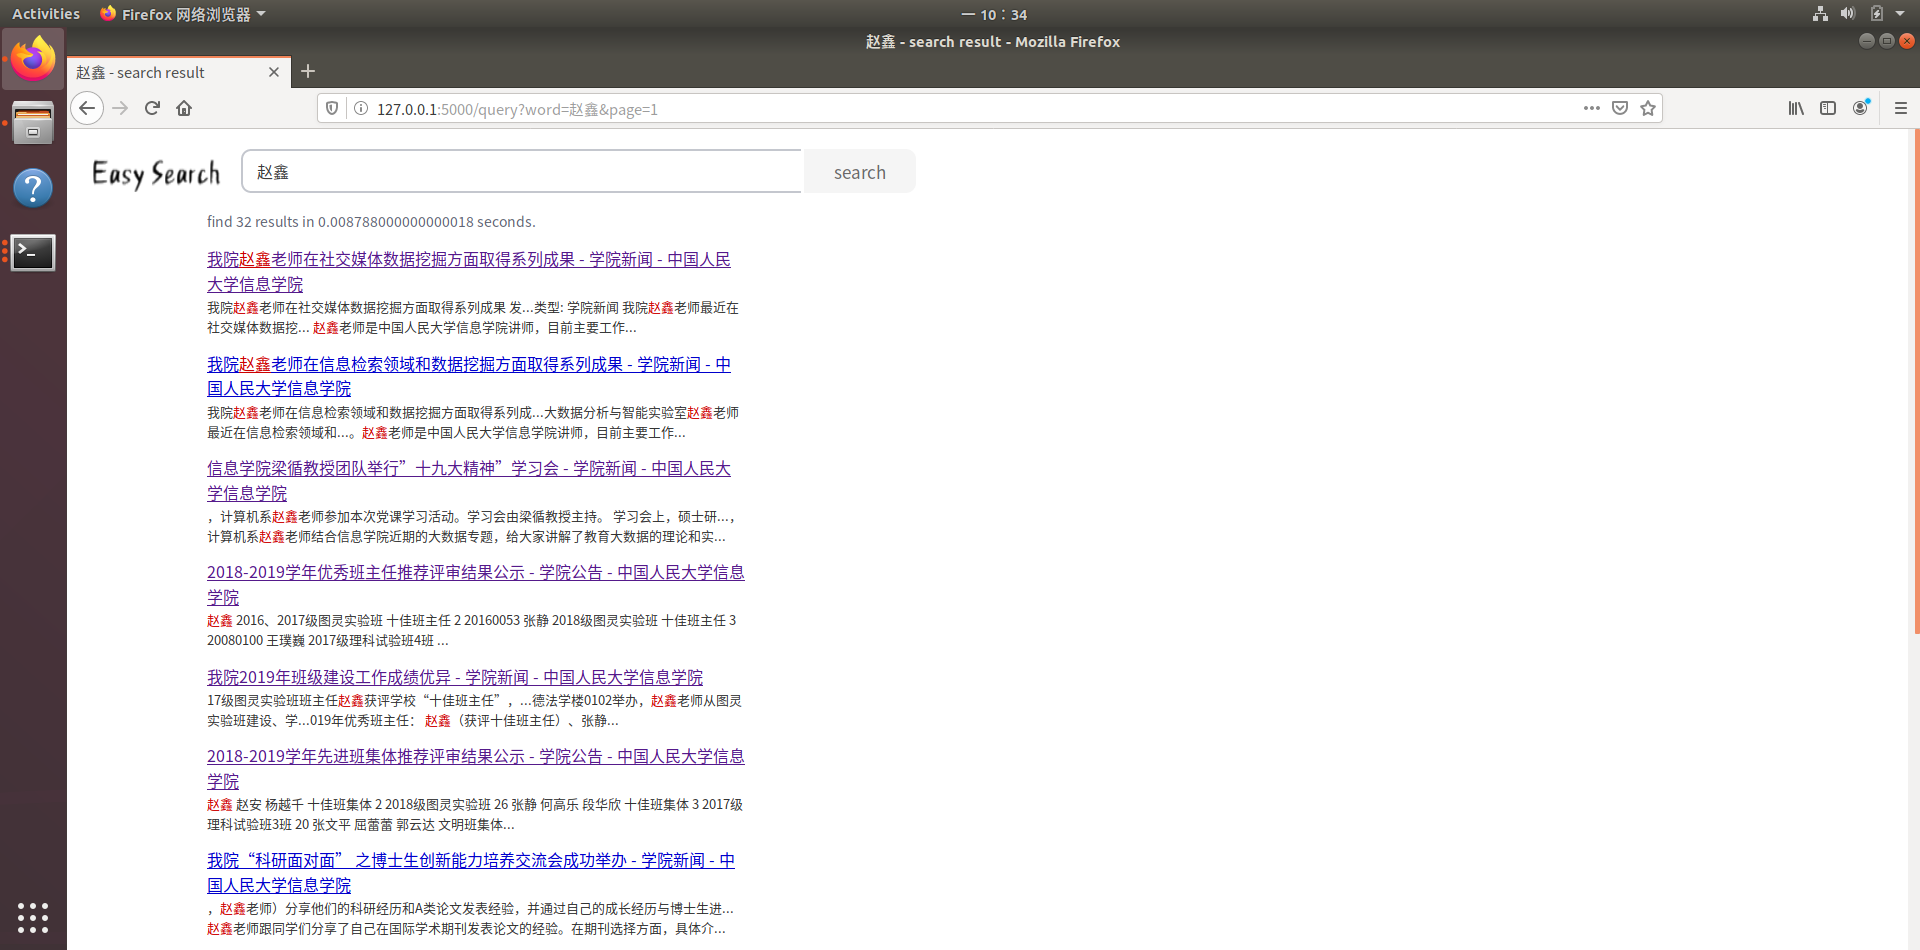
\includegraphics[height=4.5cm,width=9.5cm]{1.png}
\caption{result:part1}
\label{2}
\end{figure}

\begin{figure}[H]
\centering
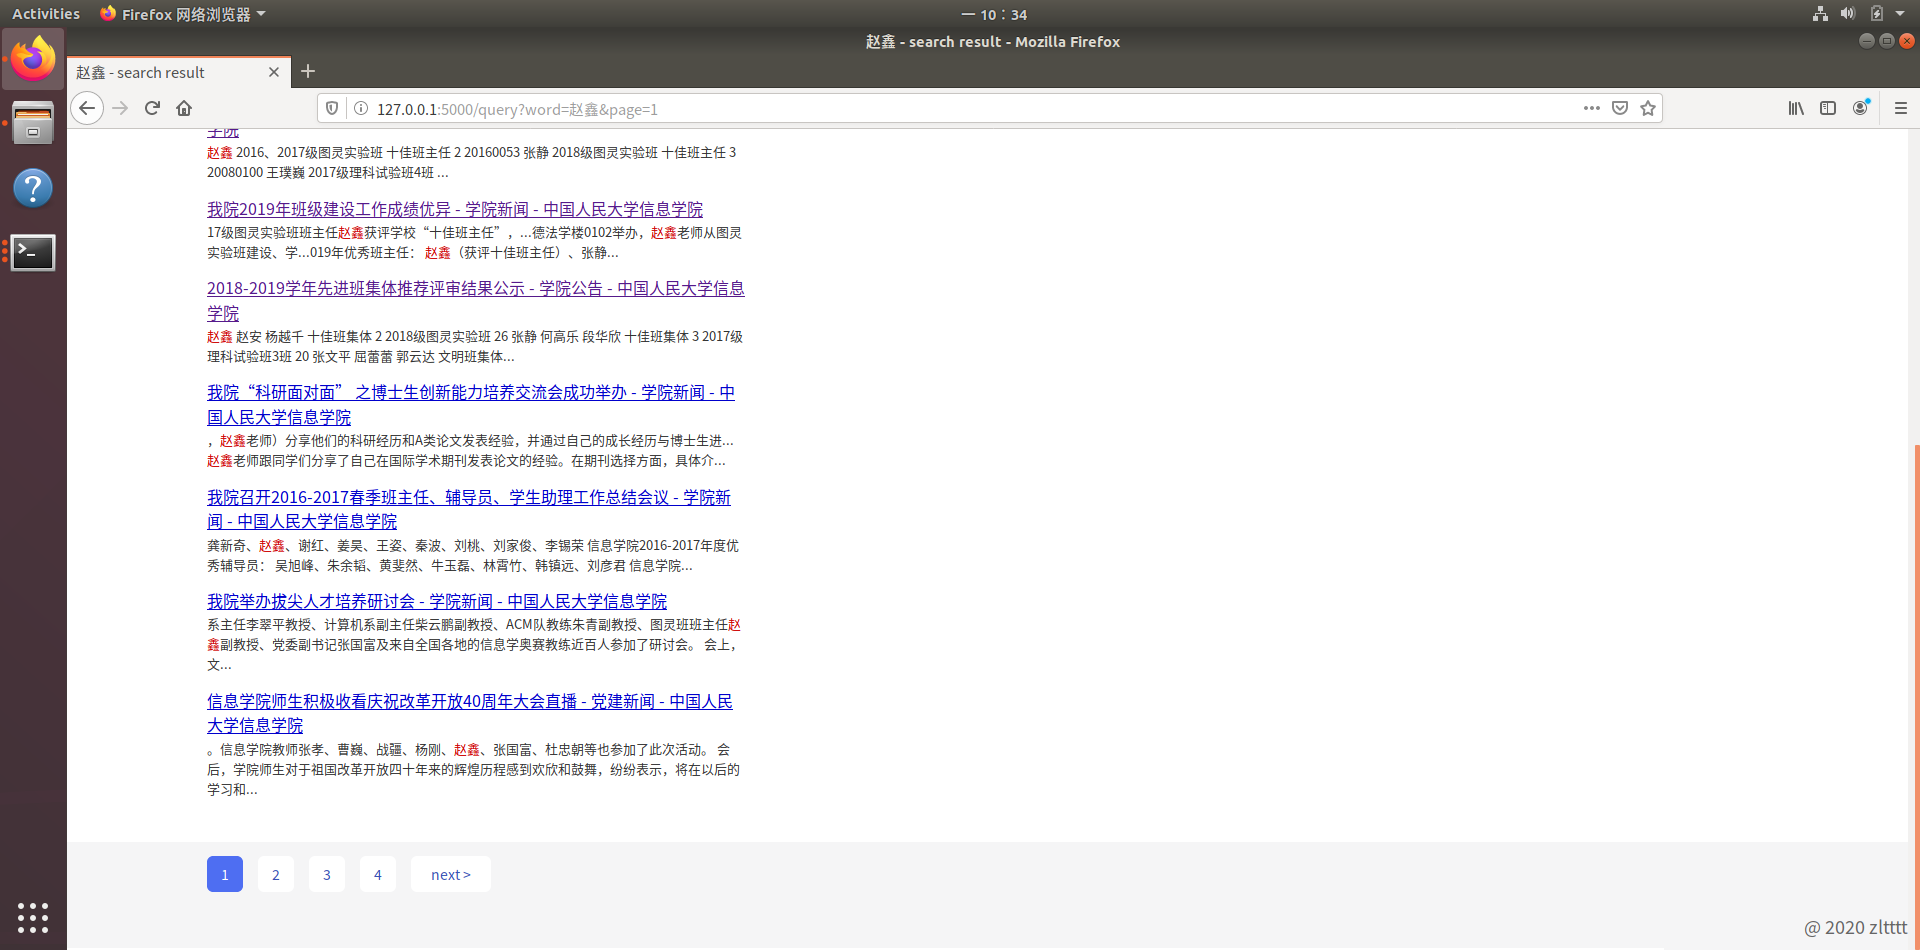
\includegraphics[height=4.5cm,width=9.5cm]{2.png}
\caption{result:part2}
\label{2}
\end{figure}

The search engine can deal with many queries like this, and can make sure that the results are reasonable. 

\section{Summary}

The engine basically achieved the goal of the SummerProgramming Lesson, and I've learned plenty of new knowledges due to the learning and designing process of this search engine. I think it is a pretty useful experience.

\section{How to use}

\subsection{Requirements}

\begin{itemize}
\item Python3
\item Flask (\url{https://palletsprojects.com/p/flask/})
\item Jieba (\url{https://github.com/fxsjy/jieba})
\end{itemize}

\subsection{Usage}

If it is the first time to start it, edit "app/target\_website.txt", and change the website link inside to your target website, and the initial value will be "http://info.ruc.edu.cn". Then run "app/initialize.py" using command "python3 initialize.py", and wait until the initialization progress finished.

To start the engine, use command "python3 -m flask run" at base directory, then use a browser to access the link provided by flask to visit the engine's main page.

\end{document}